\documentclass[12pt,titlepage]{article}
\usepackage[dvipsnames,rgb,dvips,table]{xcolor}
\usepackage{graphicx}
\usepackage[font=small,labelfont=bf]{caption}
\graphicspath{{../Figures/}}
\usepackage{psfrag}
\usepackage{dcolumn}
\usepackage{bm}
\usepackage{amsmath}
\usepackage{amssymb}
\usepackage[rflt]{floatflt}
\usepackage{latexsym}
%\usepackage{float}
\usepackage{bm}
\usepackage{subcaption}
\usepackage{booktabs}
\usepackage{floatrow}
\floatsetup[table]{font=footnotesize}
\usepackage[hidelinks]{hyperref}
\usepackage{array}
\usepackage{ragged2e}
\newcolumntype{P}[1]{>{\RaggedRight\hspace{0pt}}p{#1}}
\usepackage{color}
\usepackage[bottom]{footmisc}

\usepackage[left=20mm,right=20mm,top=25mm,bottom=20mm]{geometry}


\pagestyle{myheadings}
\markright{{\small Jacopo Credi \hfill (910216-T396) \,}}
\DeclareMathOperator\erf{erf}
\author{Jacopo Credi \\(910216-T396) \\ \vspace*{2cm} }
\title{{\Large \textsc{Chalmers University of Technology}} \\ \bigskip FFR135 - Artificial Neural Networks\\ \bigskip Examples sheet 4 \\ \vspace*{2cm}}

\usepackage{listings}
\usepackage{color} %red, green, blue, yellow, cyan, magenta, black, white
\definecolor{mygreen}{RGB}{28,172,0} % color values Red, Green, Blue
\definecolor{mylilas}{RGB}{170,55,241}
% Settings for writing Matlab code
\lstset{language=Matlab,%
	basicstyle=\small\ttfamily,
    %basicstyle=\color{red},
    breaklines=true,%
    morekeywords={matlab2tikz},
    keywordstyle=\color{blue},%
    morekeywords=[2]{1}, keywordstyle=[2]{\color{black}},
    identifierstyle=\color{black},%
    stringstyle=\color{mylilas},
    commentstyle=\color{mygreen},%
    showstringspaces=false,%without this there will be a symbol in the places where there is a space
    numbers=left,%
    numberstyle={\tiny \color{black}},% size of the numbers
    numbersep=9pt, % this defines how far the numbers are from the text
    %emph=[1]{for,end,break},emphstyle=[1]\color{red}, %some words to emphasise
    frame=single,                   % adds a frame around the code
  	rulecolor=\color{black},
    %emph=[2]{word1,word2}, emphstyle=[2]{style},    
}


\setlength{\parskip}{3pt}

\begin{document}
\parindent=0cm
\maketitle

\subsection*{Task 1a}

\begin{figure}[htbp]
\centering
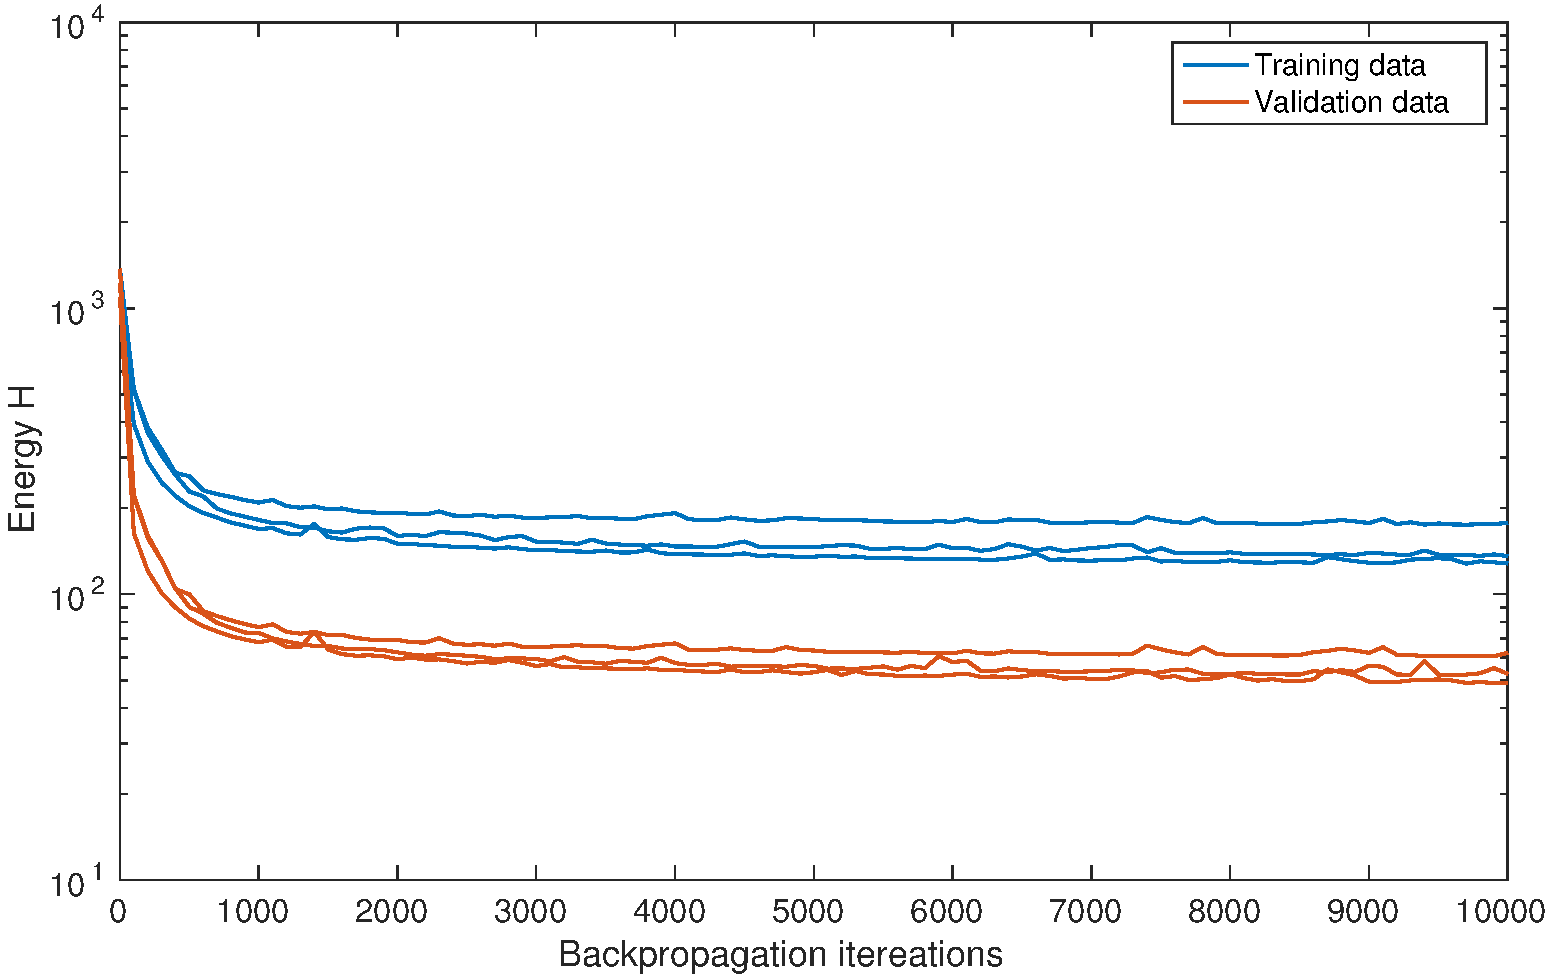
\includegraphics[width=0.75\textwidth]{1a_energy.pdf}
\caption{Energy (in log scale) vs iterations of backpropagation algorithm, for $N_G = 5$ Gaussian nodes. Training data in blue, validation data in red. For clarity, only three runs out of 20 are shown, each with only one point every 100 iterations. Parameters in the competitive learning phase: $10^5$ iterations, learning rate $\eta_c = 0.02$, neighbourhood function width $\sigma = 0.1$. Parameters in the backpropagation phase: $10^4$ iterations, learning rate $\eta_b = 0.1$, activation function $g(b) = \tanh(\beta b)$, with $\beta = 0.5$.}
\label{1a_energy}
\end{figure}

The provided data were classified using a neural network which combines unsupervised (competitive learning) and supervised learning (simple perceptron).
For the competitive learning part, $N_G = 5$ Gaussian nodes were used. Given an input vector\footnote{In this case, the data need not be normalised because we are not going to pass them (directly) through a sigmoid function, and there is no risk of zero derivative as in the perceptron case.} $\bm{x}^{\mu}$, the winning neuron (denoted by $i_0$) is the unit whose activation function is maximum: $g_{i_0}(\bm{x}^{\mu}) \geq g_{i}(\bm{x}^{\mu})$ for all $i = 1,\ldots,N_G$. After determining the winning unit, all weights are updated, according to the following learning rule:
\[
\delta \bm{w}_i \ = \ \eta \ \Lambda(i,i_0) \ (\bm{x}^{\mu}-\bm{w}_i) \ ,
\]
where the neighbouring function $\Lambda(i,i_0)$ was taken to be $\Lambda(i,i_0) = \exp{[-||i-i_0||^2/(2\sigma^2)]}$. Then, the Gaussian nodes are used as input units of a simple perceptron, trained with backpropagation. In order to do this, the data were randomly divided in two parts: one for training (70\%) and
the other for validation (the remaining 30\%).

Figure~\ref{1a_energy} shows the energy change as the backpropagation training is carried out. The energy quickly drops by a factor of $\sim8$ in the first 2000 iterations, but then does not decrease further. The average final energy, with parameters in figure caption and $N_G = 5$ Gaussian nodes, is
\[
H_{\textup{training}}^{\textup{final}} = (14 \pm 2)\cdot 10^1, \qquad \mbox{and} \qquad H_{\textup{validation}}^{\textup{final}} = (6.0 \pm 1.1)\cdot 10^1
\]
Values are averages over 20 runs, with standard deviation. The ratio of the values reflect the size of the two datasets, as energy is extensive. We will later see (\textbf{2a}) that such values correspond to a rather poor classification performance.

\clearpage
\subsection*{Task 1b}

Final classification error (training set): 0.069, uncertainty: 0.010
  Final classification error (validation set): 0.070, uncertainty: 0.014
  
  
\clearpage

\appendix

\subsection*{\texttt{UpdatePlots.m}}

\begin{lstlisting}
function [] = UpdatePlots(tPlot, trainingErrorHandle, trainingError, ...
    validationErrorHandle, validationError, trainingEnergyHandle, ...
    trainingEnergy, validationEnergyHandle, validationEnergy)
%UPDATEPLOTS

plotTrainingError = get(trainingErrorHandle,'YData');
plotTrainingError(tPlot) = trainingError;
set(trainingErrorHandle,'YData', plotTrainingError);

plotValidationError = get(validationErrorHandle,'YData');
plotValidationError(tPlot) = validationError;
set(validationErrorHandle,'YData', plotValidationError);

plotTrainingEnergy = get(trainingEnergyHandle,'YData');
plotTrainingEnergy(tPlot) = trainingEnergy;
set(trainingEnergyHandle,'YData', plotTrainingEnergy);

plotValidationEnergy = get(validationEnergyHandle,'YData');
plotValidationEnergy(tPlot) = validationEnergy;
set(validationEnergyHandle,'YData', plotValidationEnergy);

drawnow;

end
\end{lstlisting}


\end{document}